\section{Least squares approximation}
Consider, with $n > p$: 
\[
    X \in \mathbb{R}^{n \times p} \hspace{1cm} n = \text{\# samples}, \hspace{0.1cm} p = \text{\# features}, \text{ rank(}X\text{)} = p   
\]
\[
    \underline{y} \in \mathbb{R}^n \hspace{1cm} \text{labels of each sample}    
\]
We have:
\[
\underbrace{
\begin{bmatrix}
    \horzbar & \underline{x_1^\intercal} & \horzbar\\
    \horzbar & \underline{x_2^\intercal} & \horzbar\\    
     & \vdots & \\
    \horzbar & \underline{x_n^\intercal} & \horzbar
\end{bmatrix}}_{p}
\hspace{1cm}
\underbrace{x_j}: \text{j-th column of \emph{X}}
\]
If we provide a new sample $\tilde{\underline{x}} \rightarrow \tilde{y}$ we want to predict $\tilde{y}$, i.e. the label, using the information we have from the training set.\\
We can use a linear model:
\[
    \tilde{y} = \tilde{\underline{x}}^\intercal \underline{w} \hspace{1cm} \underline{w} \in \mathbb{R}^p
\]
Typically $\underline{y} \neq X\underline{w}$ so $\underline{y}$ won't be precisely obtained with that multiplication. We will have to the approximation: $\hat{\underline{y}} = X\underline{w}$. So we can say that $\hat{\underline{y}} \in \mathcal{C}(X)$ while in general $\underline{y} \notin \mathcal{C}(X)$.
The error of the prediction is given by:
\[
    r_i(\underline{w}) = \underline{y_i} - \underline{\hat{y_i}}    
\] 
We define the \textbf{residual vector} as $\underline{r}(\underline{w})$ and our goal is to minimize its l2-norm squared: $||\underline{r}(\underline{w})||^2_2$.\\

Mathematically we can describe the problem as finding: $\hat{\underline{w}} = \underset{\underline{w}}{\arg\min}||\underline{r}(\underline{w})||^2_2$. There are two approaches possible:
\begin{enumerate}
    \item Geometrical interpretation
    \item By means of optimization procedures
\end{enumerate}
\subsection{Geometrical interpretation}
\begin{center}
    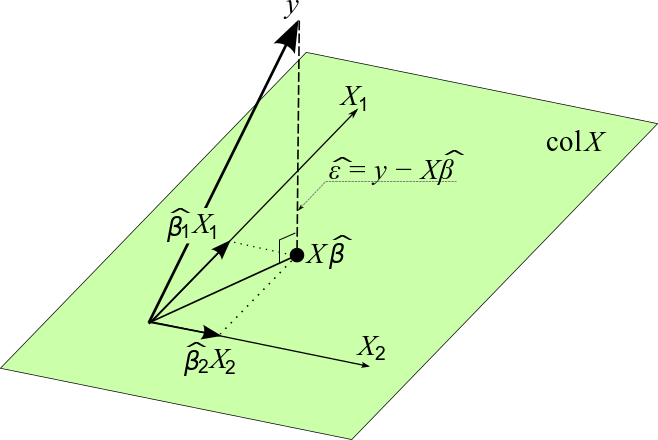
\includegraphics[scale = 0.4]{../images/OLS_geometric_interpretation.png}
\end{center}
So, a brief description of the figure above:
\begin{itemize}
    \item the plane is the space of the predictions $\mathcal{C}(X)$ indeed it is spanned by the column vectors of $X$ 
    \item the vector $\underline{y}$ is the vector of the label to be predicted
    \item the vector $X\hat{\beta}$ in the figure is our prediction $\hat{\underline{y}}$ and correspond to the projection of $\underline{y}$ on the plane $\mathcal{C}(X)$
    \item $\epsilon$ is the residual vector $\underline{r}(\underline{w})$ and represent the error between the predicted value and the actual label
\end{itemize}
If we pick $\underline{\overline{y}} \in \mathcal{C}(X)$ different from $\hat{\underline{y}}$ and their respective residuals: $\underline{\overline{r}} = \underline{y} - \underline{\overline{y}}$ and $\underline{\hat{r}} = \underline{y} - \underline{\hat{y}}$ we have that:
\[
    ||\underline{\hat{r}}||_2 \leq ||\underline{\overline{r}}||_2
\]
Indeed, $\underline{\hat{r}}$ is the orthogonal projection of $\underline{y}$ on $\mathcal{C}(X)$ and the orthogonal projection is the closest point to the vector $\underline{y}$ in the subspace $\mathcal{C}(X)$.\\
Because of this, we can also say that:
\[
    \underline{x_j^\intercal}\underline{\hat{r}} = 0 \hspace{0.5cm} j = 1, \dots, p    
\]
in matrix form:
\[
    X^\intercal \underline{\hat{r}} = \underline{0}   \implies X^\intercal (\underline{y} - \underline{\hat{y}}) = \underline{0} \implies X^\intercal (\underline{y} - X\underline{\hat{w}}) = \underline{0} \implies X^\intercal \underline{y} = X^\intercal X \underline{\hat{w}}
\]
In general the rank of the matrix $X^\intercal X$ is the same as the rank of $X$ so if $X$ is full rank then also $X^\intercal X$ is full rank and this imply that is invertible and we can find $\hat{\underline{w}}$ like this:
\[
    \hat{\underline{w}} = (X^\intercal X)^{-1}X^\intercal \underline{y}
\]
If we are using this linear model for a binary classification we have to apply to the predicted value $\hat{\underline{y}}$ a sign function in order to have the output restrained to \{-1,1\}.\\

\subsection{Optimization}
Here we exploit mathematics for solving the initial problem:
\[
    \hat{\underline{w}} = \underset{\underline{w}}{\arg\min}||\underline{r}(\underline{w})||^2_2 = \underset{\underline{w}}{\arg\min}||\underline{y} - X\underline{w}||^2_2 = \underset{\underline{w}}{\arg\min}(\underline{y} - X\underline{w})^\intercal(\underline{y} - X\underline{w}) =     
\]
\[
    = \underset{\underline{w}}{\arg\min} \bigg[\underline{y}^\intercal \underline{y} - (X\underline{w})^\intercal \underline{y} - \underline{y}^\intercal (X\underline{w}) + (X\underline{w})^\intercal X\underline{w}  \bigg]= \underset{\underline{w}}{\arg\min} \underbrace{\bigg[\underline{y}^\intercal \underline{y} - 2\underline{y}^\intercal X\underline{w} + \underline{w}^\intercal X^\intercal X\underline{w}\bigg]}_{F(\underline{w})}
\]
$F(\underline{w})$ is a \textbf{quadratic functional}. $X$ is full rank, $X^\intercal X$ is positive definite so this means that the functional is strictly convex and has a unique minimum.
So we can compute the gradient and set it to zero:
\[
    \nabla_{\underline{w}}F(\underline{w}) = -2X^\intercal \underline{y} + 2X^\intercal X\underline{w} = \underline{0}
\]
\textbf{Example 1 - Derivation}
\[
    F(\underline{w}) = \underline{w}^\intercal \underline{c} = w_1 c_1 + w_2 c_2 + w_3 c_3 = \underline{c}\underline{w}^\intercal \hspace{1cm} \underline{w}, \underline{c} \in \mathbb{R}^3    
\]
The gradient is:
\[
    \nabla F = \begin{bmatrix}
        \dfrac{\partial F}{\partial w_1}\\
        \dfrac{\partial F}{\partial w_2}\\
        \dfrac{\partial F}{\partial w_3}
    \end{bmatrix} = \begin{bmatrix}
        c_1\\
        c_2\\
        c_3
    \end{bmatrix} = \underline{c}    
\]
\textbf{Example 2 - Derivation}
\[
    F(\underline{w}) = \underline{w}^\intercal A \underline{w} = \sum_{i=1}^n \sum_{j=1}^n w_j a_{ij} w_i \hspace{1cm} A \in \mathbb{R}^{n \times n}    
\]
\[
    \dfrac{\partial}{\partial w_k}(w_j a_{ij} w_i) = \begin{cases}
        a_{ij}w_i & k=j\neq i\\
        w_j a_{ij} & k=i\neq j\\
        0 & k\neq i , k\neq j\\
        2w_k a_{ij} & k=i=j
    \end{cases}    
\]

